\chapter{Simulations}
\qquad \underline{By} : Lukas
\label{chap:sim}
\section{Engine performance simulation}
\qquad In order to simulate the engine performance, the largest single burn was simulated. As the initial burn for entering a Geostationary Transfer Orbit would require more than $900$ s of engine burn time due to the large starting mass of the spacecraft, roughly half of this initial burn was simulated. An immediate result of the requirement to limit engine burn time to $900$ s is therefore, that the first burn needs to be split into two burns. The engine simulation aims to determine thrust, acceleration, $\Delta v$ and propellant masses over time. A combined MATLAB$^{\mbox{\scriptsize{\textregistered}}}$  / Simulink$^{\mbox{\scriptsize{\textregistered}}}$  was used, calculating thrust based on following equation:
\begin{equation}
	F = \dot m \times C_F \times C^*\\
\end{equation}

with : 
$$
C^* = \frac{p_c\times A_t}{\dot{m}}
$$

and

$$
C_F = \sqrt{\frac{2\times \kappa^2}{\kappa - 1}\times \bigg(\frac{2}{\kappa + 1}\bigg)\times\bigg[1 - \bigg(\frac{p_e}{p_c}\bigg)^{\frac{\kappa - 1}{\kappa}}\bigg]} + \varepsilon\bigg(\frac{p_e-p_a}{p_c}\bigg)
$$

assuming a constant mass flow rate of $\dot{m} = 10$ kg/s. Considering a constant chamber pressure after initial start-up of $40$ bars and an exit pressure of $3900$ Pa, which was determined using RPA, a steady-state thrust of $33.6$kN was observed, as can be seen in \autoref{fig1}. $\kappa$ was determined using RPA as well and, while varying slightly throughout the engine, assumed as constant to facilitate the simulation.

\begin{figure}[H]
	\centering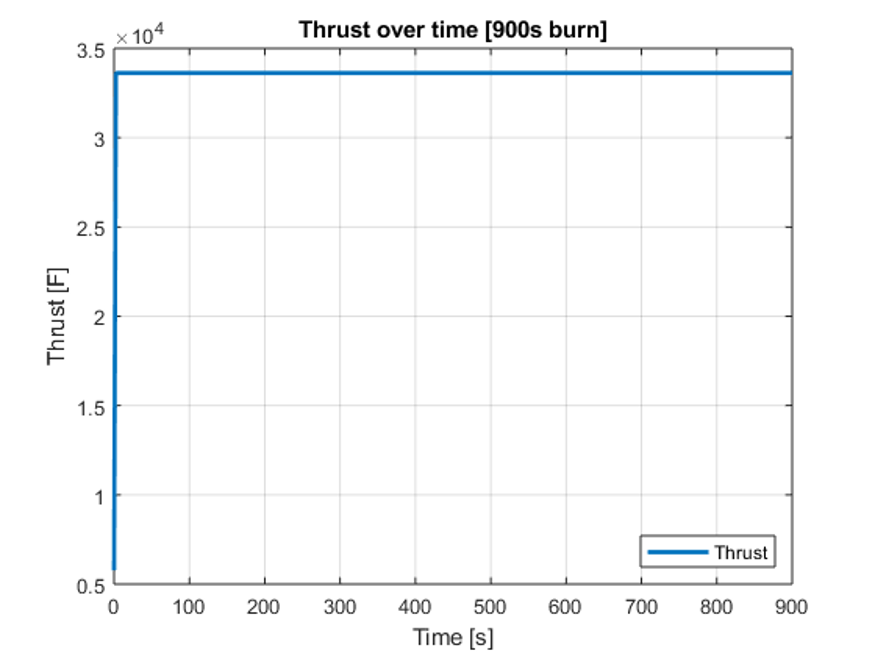
\includegraphics[width=0.9\linewidth]{thrusttime}
	\caption{Engine simulation - Thrust over time}\label{fig1}
\end{figure}

The resulting acceleration and $\Delta v$ over time are shown in \autoref{fig2}.
\begin{figure}[H]
	\centering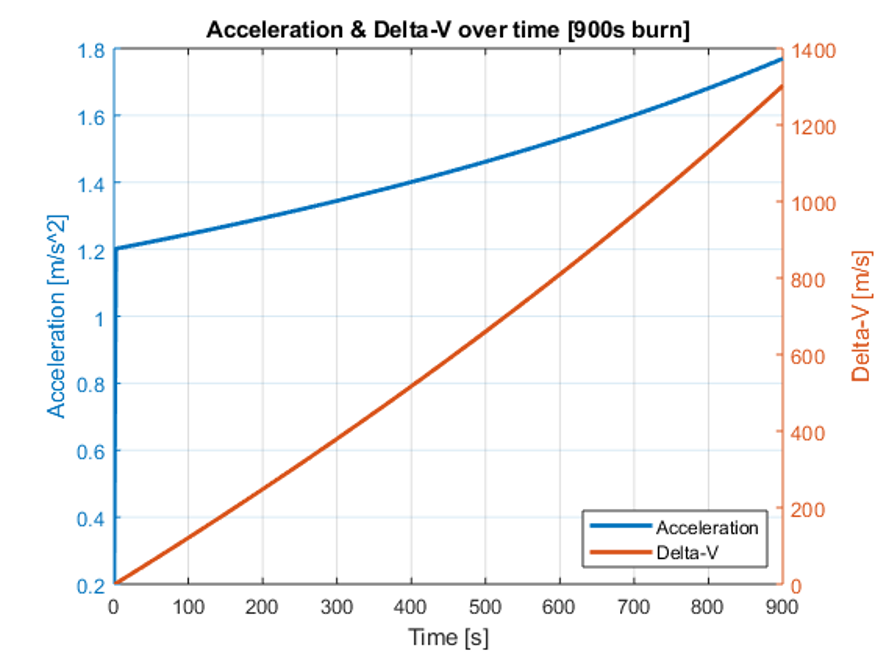
\includegraphics[width=0.9\linewidth]{accdeltav}
	\caption{Engine simulation - Acceleration and $\Delta v$ over time}\label{fig2}
\end{figure}

The acceleration, shown in blue, starts off at around $1.2$ m/s$^2$, which is a value in the range of our expectations. After $900$ seconds, the mass loss leads to a final acceleration of slightly below $1.8$ m/s$^2$, when a $\Delta v$ of ca. $1\ 300$ m/s is reached. At the point of discovery of the insufficiency of $900$ s, the decision to divide the first burn into two was taken. 
Lastly, the behavior of the propellant masses is portrayed in \autoref{fig3}. 

\begin{figure}[H]
	\centering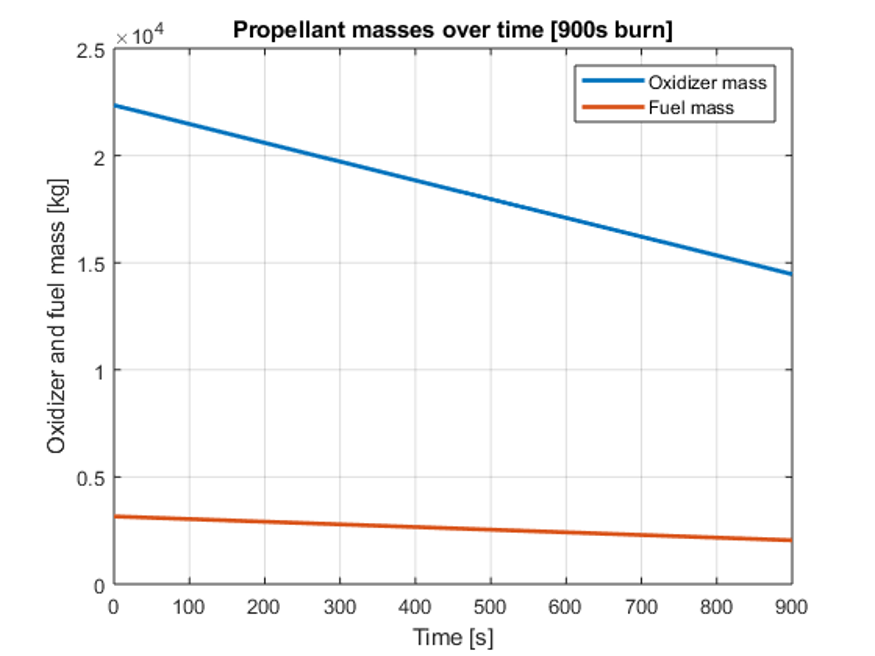
\includegraphics[width=0.9\linewidth]{propmasstime}
	\caption{Engine simulation - Propellant masses over time}\label{fig3}
\end{figure}

With roughly one third of the total usable propellant having been burnt throughout 900 seconds of burn time, these results are also according to expectations. The simulation of the maximum burn time is representative of the entirety of burns throughout the mission, therefore it validates the viability of the engine design for the fulfillment of mission requirements. The complete simulation script and model can be found in the annex. \pagebreak 
\section{Regenerative cooling simulation}

\qquad The thermal loads of the engine combustion are managed by regenerative cooling of the engine, with the cooling channels running along axial lines throughout the entire length of the engine. The cooling liquid is the engine fuel (RP-1), being fed into the combustion chamber wall and running along cooling channels with varying cross-section area before exiting at the end of the nozzle. The cooling channel design was determined by simulation of the relevant wall temperatures in steady-state operation, where a temperature at a given location does not change over time, with heat flux in and out being equal. Following assumptions and design choices were made before and during the preliminary calculations:
\begin{itemize}
	\itemsep0em 
	\item	The inner engine wall is made of copper throughout the entire engine
	\item	The outer wall is made of steel
	\item	A defined number of symmetrical rectangle-shaped cooling channels run through the engine wall, with varying cross-section to allow for higher and lower thermal flux at different sections
	\item	The cooling channels are symmetrical w.r.t. to the engine propellant flow axis
	\item	Injection into the cooling channels takes place at the combustion chamber end of the engine, in order to create larger heat transfer at more thermally stressed areas due to lower coolant temperature
	\item	\textbf{The RP-1 is assumed to not change phase during the regenerative cooling} (While this decreases simulation accuracy, too little data on high-pressure RP-1 phase change behaviour was available. The temperature does however affect the liquid’s heat capacity within the simulation)
\end{itemize}

In order to simulate the steady-state thermal behaviour of the engine along its length, some simplifications needed to be conducted. All coefficients (e.g. ratio of specific heat capacities) are assumed to be constant throughout each section, with three different values for the combustion chamber, throat area and nozzle respectively. In addition, all time-related values were transformed into distance-based values, so that the simulation time is actually millimetres, instead of seconds. This was achieved by limiting the simulation time to the engine length in millimetres and using switches to change constants based on what section the propellant is in at any given millimetre value, while using the flow velocity as the key parameter to transform into metres. The simulation script, model and complete results can be found in the annex. At this point, only some key conclusions will be presented and discussed.\\

The central aim of the iterative calculation was to determine a combination of material, wall thickness and cooling channel geometry which allows the inner wall temperature to remain below its maximum operating temperature. All other temperatures, like the coolant and outer wall temperatures, were of secondary importance. Due to its high thermal conductivity, copper was chosen as the inner wall material.

 The cooling channel cross-section was defined to always be equally sized relative to the local engine diameter, with the ratio being a function of the local engine wall cross-section area and a factor, which represents the filling grade. \autoref{fig4} shows the cross-section change over the engine length. The rectangular geometry is defined by a ratio of width to height of $5$.

\begin{figure}[H]
	\centering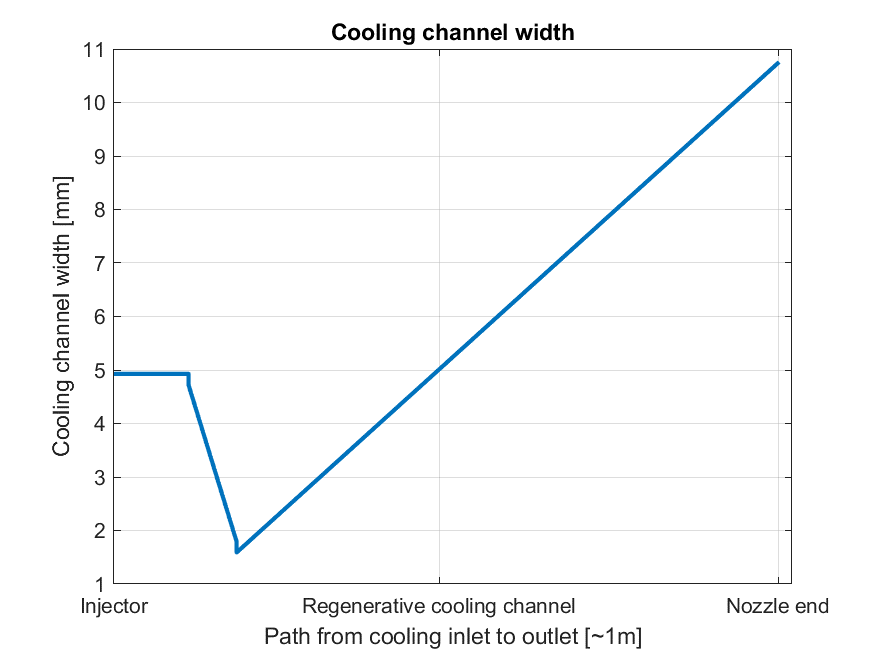
\includegraphics[width=0.9\linewidth]{coolingchannelwidth}
	\caption{Regenerative cooling simulation - Cooling channel width over engine length}\label{fig4}
\end{figure}

The final cooling channel system is a compromise between the copper wall temperature and minimum necessary material for weight savings. Therefore, the copper wall has a thickness of $6$ mm in the combustion chamber, $7$ mm in the throat area and $5$ mm in the nozzle section. The resulting relevant temperatures can be seen in \autoref{fig5}.

\begin{figure}[H]
	\centering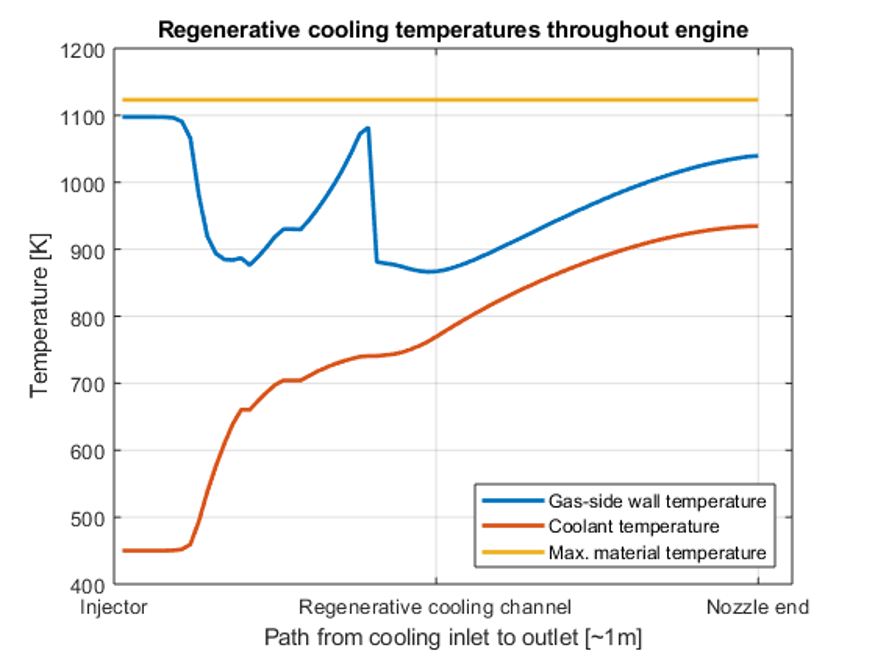
\includegraphics[width=0.9\linewidth]{relevanttemps}
	\caption{Regenerative cooling simulation - Relevant temperatures}\label{fig5}
\end{figure}

The highest temperatures can be observed in the combustion chamber section, as low flow speeds cause less convective heat transfer to take place, reducing the overall heat flux. The gas-side wall temperature then drops in the beginning of the throat area, before rising again towards the throat. After passing the throat, the gas-side wall temperature drops sharply and then rises again towards the nozzle exit.
\section{Hydrogen peroxide decomposition simulation}
\label{sec:11-3}
\qquad As mentioned in \autoref{sec:10-3}, the decomposition of hydrogen peroxide is used for self-pressurization of the oxidizer tank as well as power generation in a fuel cell in combination with hydrogen. As hydrogen peroxide is not only decomposing, but the decomposition is also an exothermal process, the thermal control system needs to be well under control in order to avoid critical behavior of the hydrogen peroxide if $150^\circ$ C are exceeded. Therefore, a detailed simulation has been performed, taking wall thicknesses, materials, radiative and absorbing coefficients as input parameters. The simulation is structured like a control system, calculating the temperature of the hydrogen peroxide inside the tank, the cold and hot wall temperatures. Upon reaching the specified target temperature, the control loop rotates the spacecraft to a neutral degree for constant hydrogen peroxide temperature. Before discussing the results, an overview of the simplifications taken for facilitation of the simulation follows:
\begin{itemize}
	\itemsep0em 
	\item	Inside the tank, only vaporization takes place, no condensation
	\item	The space craft can rotate to any angle instantaneously and there is no modelling of the necessary thruster activation
	\item	The cold and hot walls are always at a homogenous temperature, only depending on heat flux between hydrogen peroxide, the walls, the sun and dark space
	\item	As the structural calculations needed to be complete before the simulation was able to prove the technical feasibility of the decomposition regulation, \textbf{the hydrogen peroxide tank is assumed to be made of only one material throughout the rest of the documentation, while the simulation allows for two different materials}, as different heat flux coefficients are advantageous. Therefore, the results of this simulation are not exactly compatible with the final space craft design and more of a proof of concept, to be reunited with the structural design as a next step.
\end{itemize}

The simulation showed that, with the simplifications taken, a control system maintaining the hydrogen peroxide pressure at an acceptable level is technically feasible. A control reaction to raising the temperature from $310$ K to $350$ K has been chosen as the case for technical feasibility demonstration. As explained in \autoref{sec:10-3}, the rotational angle of the space craft is the dictating parameter for heat input and output. \autoref{fig6} shows the rotational angle, resulting H2O2 pressure, the relevant temperatures and the generated energy considering consumption of all generated oxygen in the fuel cell. The four graphs are outputs of the same simulation, the complete script and model for which can be found in the annex. The initial values for the integration blocks, which output temperatures, are all assumed.

\begin{figure}[H]
	\centering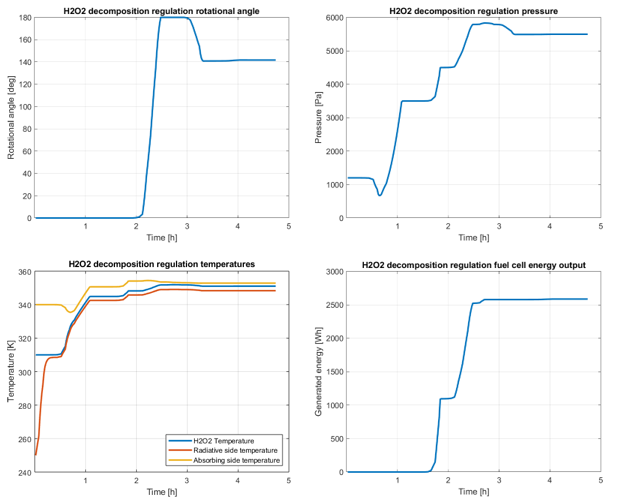
\includegraphics[width=\linewidth]{feasibility}
	\caption{Demonstration case for technical feasibility of $H_2O_2$ decomposition regulation}\label{fig6}
\end{figure}
As the simulation results show, the rotational angle is initially maintained at $0^\circ$, meaning full exposure of the more absorbing side towards the sun, with the less radiative side facing dark space. After $2$ hours, the space craft turns towards the other side, decreasing the heat flux gradually while approaching the target temperature. In the end, a constant neutral rotational angle of $140^\circ$ is maintained, with a final control error of around $1-2$ K. After this process, $2,5$ kWh of energy were generated, while the pressure inside the tank has risen from around $1000$ Pa to $5500$ Pa. The tank pressure is determined via interpolation of temperature-dependent vaporization pressures to gain a function of pressure with respect to temperature.